\begin{filecontents*}{example.eps}
gsave
newpath
  20 20 moveto
  20 220 lineto
  220 220 lineto
  220 20 lineto
closepath
2 setlinewidth
gsave
  .4 setgray fill
grestore
stroke
grestore
\end{filecontents*}
\RequirePackage{fix-cm}
\documentclass[smallextended]{svjour3}       % onecolumn (second format)

\smartqed  % flush right qed marks, e.g. at end of proof

\usepackage{graphicx}


%below is added
\usepackage{xcolor}
\usepackage{colortbl}
\usepackage{cite}
\usepackage{amsmath,amssymb,amsfonts}
\usepackage{algorithmic}
\usepackage{graphicx}
\usepackage{textcomp}
\usepackage{tabularx}
\usepackage{amsmath}
\usepackage{enumitem}
\usepackage{hyperref}
\usepackage{tikz}
\usepackage{threeparttable}
\usepackage{fancyvrb}
\usepackage{booktabs}
\usepackage[normalem]{ulem}
\usepackage{balance}
\usepackage[all]{nowidow}
\usepackage{adjustbox} 
\usepackage{lscape}

\usepackage{hyperref}
\makeatletter

%add again
\def\UrlAlphabet{%
	\do\a\do\b\do\c\do\d\do\e\do\f\do\g\do\h\do\i\do\j%
	\do\k\do\l\do\m\do\n\do\o\do\p\do\q\do\r\do\s\do\t%
	\do\u\do\v\do\w\do\x\do\y\do\z\do\A\do\B\do\C\do\D%
	\do\E\do\F\do\G\do\H\do\I\do\J\do\K\do\L\do\M\do\N%
	\do\O\do\P\do\Q\do\R\do\S\do\T\do\U\do\V\do\W\do\X%
	\do\Y\do\Z}
\def\UrlDigits{\do\1\do\2\do\3\do\4\do\5\do\6\do\7\do\8\do\9\do\0}
\g@addto@macro{\UrlBreaks}{\UrlOrds}
\g@addto@macro{\UrlBreaks}{\UrlAlphabet}
\g@addto@macro{\UrlBreaks}{\UrlDigits}
\makeatother

\usepackage{listings}
\lstset{
	breaklines=true,
	frame=single,
	label=lst1:mxm,
	basicstyle=\scriptsize\ttfamily,
	keywordstyle=\bfseries,
	stringstyle=\ttfamily\color{red!50!brown},
	numberstyle=\tiny\color{gray}\sffamily,
	xleftmargin=2em,
	basewidth={0.55em, 0.45em},
	framexleftmargin=0em,
	framexrightmargin=-0.5em,
	numbers=left,
	language=java,
	moredelim=**[is][\color{red}]{@}{@},
	moredelim=**[is][\color{green!60!black}]{~}{~},
}

% comments
\usepackage{soul,color,xspace}
\newcommand{\jyy}[1]{\sethlcolor{yellow}\hl{jyy:#1}\xspace}
\newcommand{\lwj}[1]{\sethlcolor{green}\hl{lwj:#1}\xspace}
\newcommand{\TODO}[1]{\sethlcolor{orange}\hl{TODO:#1}\xspace}

%language
%\usepackage{fontspec, xunicode, xltxtra}  


% document parts
\newcommand{\code}[1]{{\small\texttt{#1}}}
\newcommand{\smalltitle}[1]{\smallskip\noindent{\textbf{#1}}.}
\newcommand{\finding}[2]{%
	\begin{center}%
		\begin{tikzpicture}%
		\node[rectangle, draw=#1, top color=#1!5, bottom color=#1!5, rounded corners=2pt, inner xsep=5pt, inner ysep=6pt, outer ysep=10pt]{
			\begin{minipage}{0.9\columnwidth}#2\end{minipage}};%
		\end{tikzpicture}%
	\end{center}%
}

% table items
\newcommand{\rowhead}{\rowcolor{white}}
\newcommand{\odrow}{\rowcolor{gray!15}}
\newcommand{\evrow}{\rowcolor{white}}
\newcommand{\cat}[1]{{\scriptsize(#1)}}
\newcommand{\subj}[1]{#1 \rm\cite{#1}}
\newcommand{\rev}[1]{\scriptsize{\texttt{#1}}}
\newcommand{\pending}[1]{{\color{black!70}{\##1}}}
\newcommand{\reject}[1]{{\color{red}\sout{\##1}}}
\newcommand{\partrejfix}[1]{{\color{blue}{\bf\##1}%
		$^\textrm{{\color{blue}partially-fixed}/{\color{red}rejected}}$
}}
\newcommand{\confirm}[1]{{\color{blue}{\bf\##1}}}
\newcommand{\fixed}[1]{{\color{blue}{\bf\##1}$^\textrm{fixed}$}}

\renewcommand{\footnoterule}{
	\kern -3pt
	\hrule width 2in
	\kern 2.6pt
}


%end the add



%
% \usepackage{mathptmx}      % use Times fonts if available on your TeX system
%
% insert here the call for the packages your document requires
%\usepackage{latexsym}
% etc.
%
% please place your own definitions here and don't use \def but
% \newcommand{}{}
%
% Insert the name of "your journal" with
% \journalname{myjournal}
%
\begin{document}

\title{Characterizing and Detecting Inefficient Image	Displaying Issues in Android Apps}

\author{Wenjie Li         \and
	Yanyan Jiang         \and
	Chang Xu         \and
	Yepang Liu         \and
	Xiaoxing Ma         \and
    Jian Lyu %etc.
}


\institute{Wenjie Li, Yanyan Jiang, Chang Xu, Xiaoxing Ma, Jian Lyu   \at
              State Key Lab for Novel Software Technology, Nanjing University, Nanjing, China \\
              \email{wenjielinju@gmail.com, {jyy, changxu}@nju.edu.cn, {xxm, lj}@nju.edu.cn}           %  \\
%             \emph{Present address:} of F. Author  %  if needed
           \and
           Yepang Liu \at
           Shenzhen Key Laboratory of Computational Intelligence, Department of Computer Science and Engineering, Southern University of Science and Technology, Shenzhen, China\\
           \email{liuyp1@sustc.edu.cn}
}

\date{Received: date / Accepted: date}


\maketitle

\begin{abstract}
Mobile applications (apps for short) often need to display images. However, inefficient image displaying (IID) issues are pervasive in mobile apps, and can severely impact app performance and user experience.
This paper presents an empirical study of 162 real-world IID issues collected from 243 popular open-source Android apps,
validating the presence and severity of IID issues,
and then sheds light on these issues' characteristics to support future research on effective issue detection. Based on the findings of this study, we developed a static IID issue detection tool TAPIR and evaluated it with real-world Android apps. The experimental evaluations show encouraging results: TAPIR detected 43 previously-unknown IID issues in the latest version of the 243 apps, 16 of which have been confirmed by respective developers and 13 have been fixed.
\keywords{Android app \and inefficient image displaying \and performance \and empirical study \and static analysis}

\end{abstract}

\section{Introduction}

Media-intensive mobile applications (apps for short) must carefully implement their CPU- and memory-demanding image displaying procedures.
Otherwise user experiences can be significantly affected~\cite{handle_image}.
For example, inefficiently displayed images can lead to app crash, UI lagging, memory bloat, or battery drain,
and finally make users abandon the concerned apps even if they are functionally perfect~\cite{performance}.

In this paper, we empirically found that mobile apps often suffer from
\emph{inefficient image displaying} (IID) \emph{issues}
in which the image displaying code contains non-functional defects that cause performance degradation or even more serious consequences, such as the app crashing or no longer responding.
Despite the fact that existing work has considered IID issues to some extent
(within the scope of general performance bugs~\cite{liu2014characterizing,carette2017investigating, wang2016profiling, linares2015developers, Liu:SW15} or image displaying performance analysis~\cite{kwon2013mantis,gao2017every}),
there still lacks a thorough study of IID issues for mobile apps,
particularly for source-code-level insights that can be leveraged in program analysis for automated IID issue detection or even fixing.

To facilitate deeper understanding of IID issues,
this paper presents an empirical study towards characterizing IID issues in mobile apps.
We carefully localized 162 IID issues (in 36 apps) from 1,826 issue reports and pull requests in 243 well-maintained open-source Android apps in F-Droid~\cite{f-droid}. Useful findings include:

\begin{enumerate}
  \item Most IID issues cause app crash (30.9\%) or slowdown (45.1\%), and handling lots of images and/or large images are the primary causes.
  This finding is useful for developing reasonable workloads and test oracles for dynamic manifestation and detection of IID issues in Android apps.
  \item A few root causes have covered most (90.1\%) examined IID issues: non-adaptive image decoding (45.1\%), repeated and redundant image decoding (26.5\%), UI-blocking image displaying (11.1\%), and image leakage (7.4\%). We also extracted sufficient conditions for localizing these issues in an Android app's execution trace, which would benefit both dynamic and static analyzers.
  \item Certain anti-patterns can be strongly correlated with IID issues: image decoding without resizing (23.4\%), loop-based redundant image decoding (22.2\%), image decoding in UI event handlers (11.1\%), and unbounded image caching (4.3\%).
  This finding lays the foundation of our pattern-based lightweight static IID issue detection technique.
  \item \TODO{add other findings}
\end{enumerate}

To the best of our knowledge,
this paper presents the first systematic empirical study of IID issues in real-world Android apps,
and provides key insights on understanding, detection, and fixing of IID issues. 

Based on these findings,
we design and implement TAPIR, a static analyzer for IID issue detection in Android apps.
We experimentally validated the effectiveness of TAPIR, and applied it to the latest versions of all 243 studied apps.
TAPIR reported surprisingly encouraging results that 43 \emph{previously-unknown} IID issues in 16 apps (24 of the 43 issues are from eight apps that previously suffered from IID issues) were manually confirmed as true positives and reported to respective developers,
among which 16 have been confirmed by the developers and 13 have been fixed.

In summary, our paper makes the following contributions:

\begin{enumerate}
	
  \item We conducted a systematic empirical study of IID issues in real-world Android apps. The findings provide key insights to facilitate future research, and our dataset of IID issues are publicly available for follow-up studies%
\footnote{\url{https://github.com/IID-dataset/IID-issues}.}.

  \item For a more intuitive presentation and understanding of IID issues, we extracted IID issues' code slices and graphically represented them in a standard format. The graphical representation of IID issues are publicly available%
\footnote{\url{https://github.com/IID-dataset/IID-issues-graphical-representation}.}.
  
  \item Based on our empirical findings, we devised a static pattern-based IID issue detection technique, TAPIR, and validated its effectiveness using real-world Android apps.
\end{enumerate}

In our preliminary conference version of this work~\cite{li2019characterizing} , we conducted an empirical study on 162 IID issues and designed TAPIR to detect potential IID issues in Android apps. In this journal version, we extended our previous work from the following perspectives:(1)We extracted 162 IID issues' code slices and graphically represented them in a standard format. (2)We extended answers to our research questions (i.e., RQ1, RQ2, and RQ3) based on further empirical study results. (3)We additionally studied and answered two important research questions (i.e., RQ4 and RQ5) to provide a more comprehensive understanding for IID issues. (4) We provided more details of the empirical study, issue examples, technique design, and experimental setup.

The rest of this paper is organized as follows. Section~\ref{sec:background} introduces the background knowledge of image displaying in Android apps. Section~\ref{sec:study} presents the methodology of our empirical study for IID issues in Android apps and discusses our empirical findings. Section~\ref{sec:detection} presents the design and implementation of our TAPIR tool. Section~\ref{sec:evaluation} experimentally evaluates TAPIR with popular and open-source Android apps and discusses its results and the threats to validity. Section~\ref{sec:related-work} presents related work, and Section~\ref{sec:conclusion} concludes this paper.\TODO{need to be updated}


\section{Background} \label{sec:background}

Image displaying, although seemingly straightforward, is actually a non-trivial process in Android apps and can be subject to various performance defects.
In this section we introduce the image displaying process in Android apps and its related inefficient image displaying (IID) issues.

% Image displaying is very common in Android apps, which is a very important carrier of information transmission. When an image is displayed in an Android app, it can cause high computational resources overhead (e.g., CPU and RAM) and involves various and complex steps, especially when the concerned image is large. In this section, we describe the resource consumption and the process of image displaying in Android apps.   
%jyy's comments: {I don't think a long introduction is very necessary here. If we have space, we can add it back later.}

\subsection{Image Displaying in Android Apps}

The process of image displaying in Android apps consists of the following four phases, which are all performance-critical and energy-consuming~\cite{handle_image}:

\begin{itemize}  
  \item \emph{Image loading} for reading the external representation of an image (from an external source, e.g., a URL, file, or input stream) and decoding the image into an Android-recognizable in-memory object (e.g., \code{Bitmap}, \code{Drawable}, and \code{BitmapDrawable}).

  \item \emph{Image transformation} for post-decoding image processing, in which a decoded image object is resized, reshaped,
  or specially processed for fitting in a designated application scenario (e.g., a cropped and enhanced thumbnail).

  \item \emph{Image storage} for managing a decoded and/or transformed image object, particularly in a cache, for later rendering.
  Caching can also save precious CPU/GPU cycles for image decoding and transformation, but it would incur significant space overhead.
  \item \emph{Image rendering} for physically displaying an image object on an Android device's screen.
  Images are rendered natively by the Android framework~\cite{Android_framework}.
\end{itemize}

\subsection{Inefficient Image Displaying (IID)}

Image displaying is both computation- and memory-intensive. Displaying a full resolution image on a high-resolution display may cost:

\begin{itemize}
  \item hundreds of milliseconds of CPU \emph{time}~\cite{wang2016profiling}, which can cause an observable lag, and
  \item tens of megabytes of \emph{memory}~\cite{image_size}, which can drain an app's limited memory.
\end{itemize}

Therefore, the efficiency of image displaying on CPU- and memory-constrained mobile devices is of critical importance.
Inefficiently displayed images can severely impact app functions or user experiences:

\begin{enumerate}
  \item Decoding images in the UI thread can significantly degrade an app's performance, causing its slow responsiveness or even ``app-not-responding'' anomalies%
\footnote{\url{https://github.com/wordpress-mobile/ WordPress- Android/issues/5777}.}.
  \item Image objects not being freed in time can consume significantly large amounts of memory, leading to \code{OutOfMemoryError} and unexpected app terminations%
\footnote{\url{https://github.com/AnimeNeko/Atarashii/issues/6}.}.
  \item Improperly stored (cached) images may cause repeatedly (and unnecessary) processing of the same images, resulting in meaningless performance degradation and energy waste%
\footnote{\url{https://github.com/TeamNewPipe/NewPipe/pull/166}.}.
\end{enumerate}

We thus define an \emph{inefficient image displaying} (IID) issue as a non-functional defect in an Android app's image displaying implementation (e.g., improper image decoding) that causes performance degradation (e.g., GUI lagging or memory bloat) and even more serious consequences (e.g., app crash).

To better understand and detect IID issues,
in this paper we conduct an empirical study to systematically investigate IID issues in Android apps,
and work for automated IID issue detection technique based on our empirical study results.

\section{Empirical Study}\label{sec:study}

\subsection{Methodology}

Our empirical study follows a methodology similar to those adopted in existing work~\cite{liu2016understanding, hu2018tale} for characterizing real-world Android app bugs.
We extracted a set of 162 real-world IID issues by keyword search and manual inspection from 243 well-maintained open-source Android apps of realistic usage in F-Droid~\cite{f-droid} using the process in Section~\ref{subsec:dataset-collection}. We further analyzed these issues by the methodology in Section~\ref{subsec:issue-analysis}.

\subsubsection{Dataset collection} \label{subsec:dataset-collection}

We conducted the empirical study based on a collection of IID issues from Android apps. Figure~\ref{fig:issue_collection} illustrates the overall issue collection process.

\begin{figure}[ht]
  \centering
  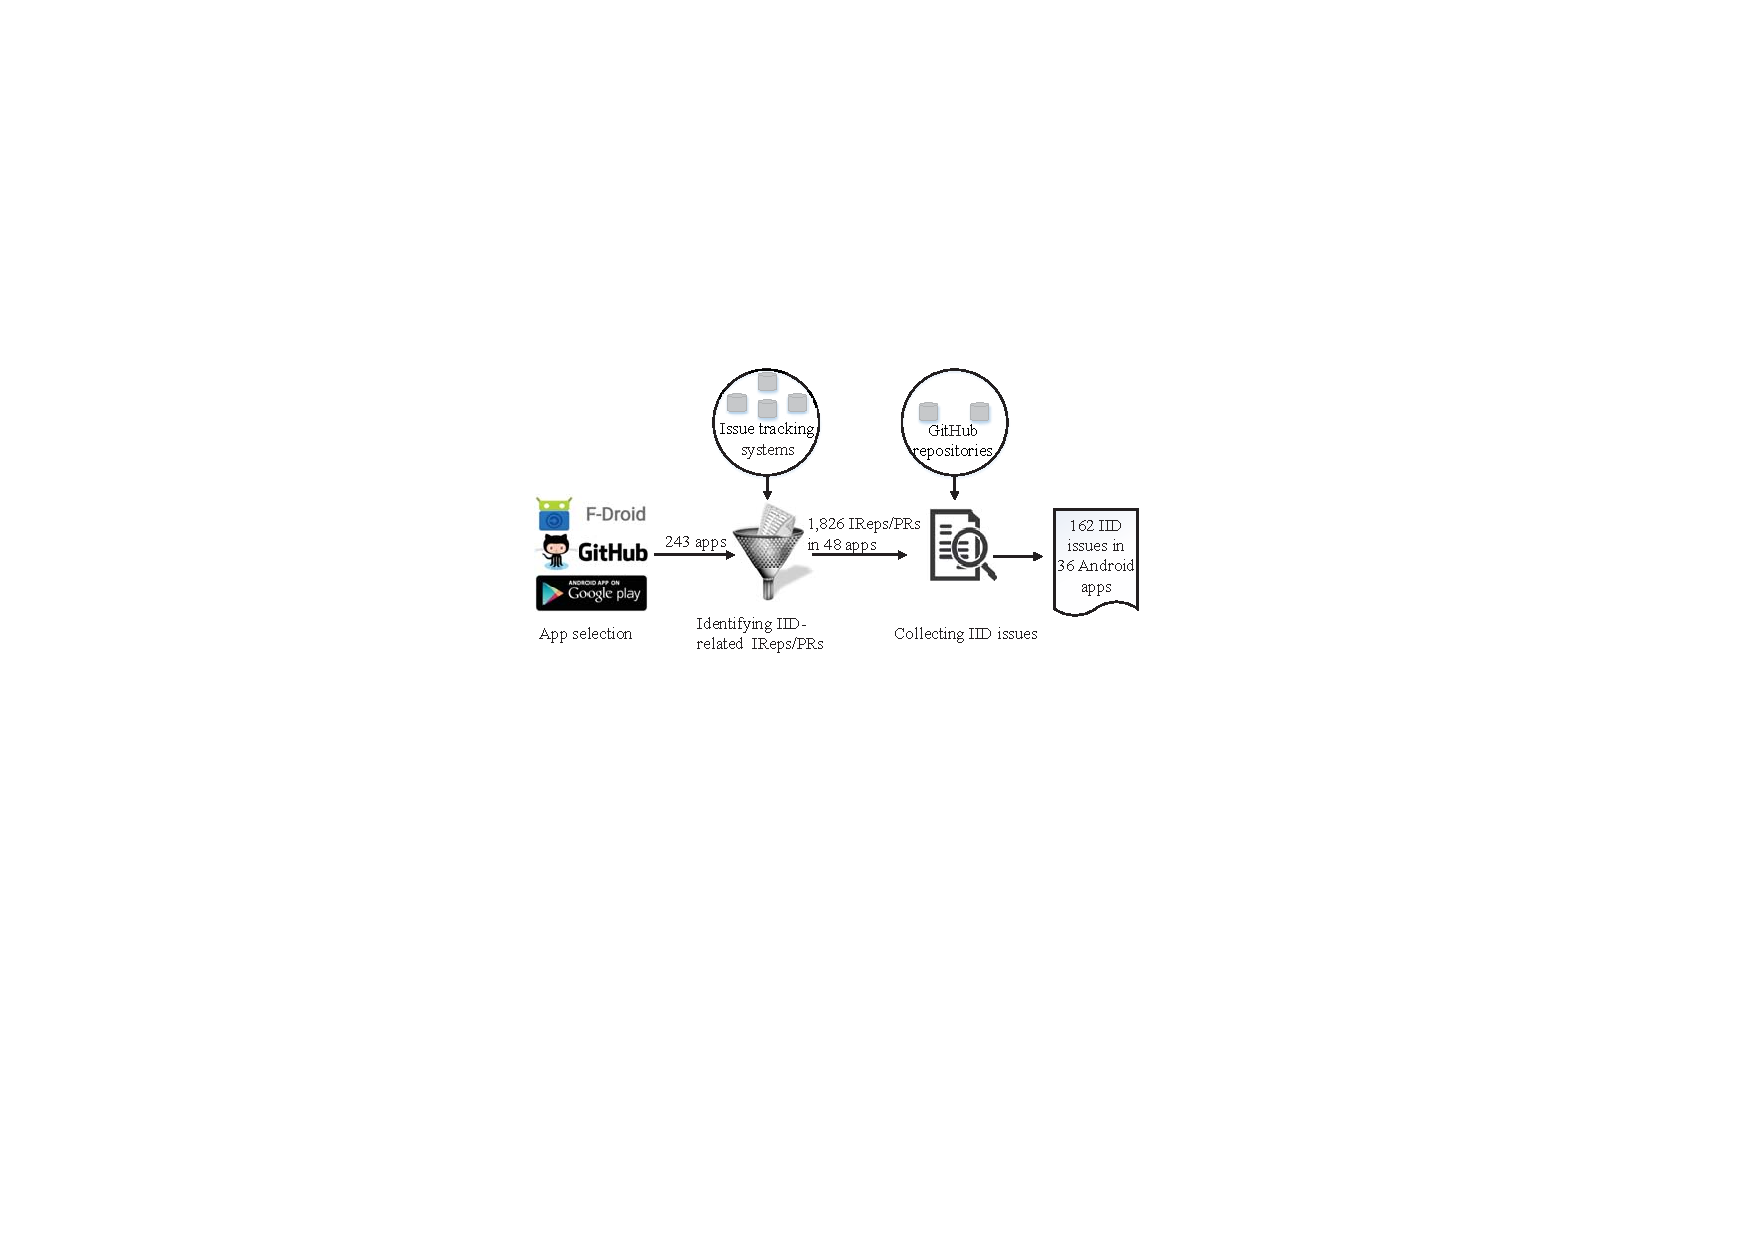
\includegraphics[scale=0.8]{pictures/fig1}
  \caption{The IID issue collection process}
  \label{fig:issue_collection}
\end{figure}

\noindent\textbf{App selection.} We selected all 243 Android apps from 1,093 randomly selected Android apps in F-Droid~\cite{f-droid} as our study subject, meeting the following selection criteria:

\begin{enumerate}
	\item \emph{Open-source}: also hosted on GitHub with an \emph{issue tracking system} for tracing potential IID issues.
	\item \emph{Well-maintained}: having over 100 code commits in the corresponding GitHub repository.
	\item \emph{Of realistic usage}: having over 1,000 downloads on the Google play market.
\end{enumerate}

\medskip

\noindent\textbf{Identifying IID-related issue reports and pull requests.}
An app user's \emph{issue report} (IRep for short) usually denotes a manifested app bug from end users.
An app developer's \emph{pull request} (PR for short), on the other hand, possibly contains the developer's perspective on a concerned app bug. Therefore, we collected both of them in the empirical study.
We first identified potential IID-related IReps and PRs in the GitHub repositories by a keyword search in their issue tracking systems using the following keywords%
\footnote{These keywords are general natural language words related to image displaying. They come from existing research work, e.g.,~\cite{linares2015developers, wang2016profiling} and our empirical study experience.}:

\begin{Verbatim}[fontsize=\small]
image   bitmap     decode   display
picture photograph show   thumbnail
\end{Verbatim}

Any IRep or PR that contains one of the above keywords in its title, body, or comment was then manually inspected to further confirm whether it indeed \emph{fixed any performance bug}:

\begin{enumerate}
  \item The IRep's/PR's text complains about the performance degradation or more serious consequences (e.g., app crash) when performing image displaying.
  \item There is evidence that an image-related bug is fixed (e.g., the concern issue report is associated with a fixing commit ID or an accepted fixing patch), and the same issue has never been re-reported in the following three months%
  \footnote{For those issues that do not contain any explicit link to any patch, we conducted a bisect on their GitHub repositories to find potential fixing patches by following the methodology of existing work~\cite{traceability}.}.
\end{enumerate}

After the manual inspection, we obtained a total of 1,826 IReps/PRs in 48 apps, which are from 22,023 IReps/PRs returned by the keyword search from the initially selected 243 Android apps.

\medskip

\noindent\textbf{Collecting IID issues and their patches.} 
We then inspected the GitHub commits associated with the 1,826 IReps/PRs to decide whether they correspond to IID issues.
For each code patch (may patch several places or files in the concerned repository, and a commit may also contain several patches) for fixing a particular image-displaying-related performance bug that is clearly documented in the corresponding IReps/PR, we consider this patch related to a new IID issue.
As such, for each decided IID issue, we obtained a patch for fixing it and its textual descriptions in the corresponding IRep/PR, which would suffice for our further manual inspection in order to answer research questions in this study.

Finally, we collected a total of 162 IID issues (distributed in 71 IReps/PRs) in 36/243 (14.8$\%$) studied Android apps. These numbers (162 issues and 14.8\% coverage) suggest that IID issues are definitely not rare, and can be considered as common in practice and deserving an in-depth study.

\medskip

\noindent\textbf{Extracting IID issues’ code slices.(\TODO{Need to be rewritten})} 
We extracted all 162 IID issues' code slices to get a deeper understanding of them from the perspective of the whole execution process of image displaying. An IID issue's code slice is a subset of statements that directly or indirectly influence the execution of inefficient image displaying through chains of dynamic data and control dependencies, which can help users focus their attention on a subset of program statements which are responsible for the issue. The process of extracting IID issues' code slices consist of following steps:

\begin{enumerate}
	\item Obtaining the IID issue’s buggy code.
	\item Obtaining the IID issue’s issue-triggering context information based on its issue description in its related issue report and comments.
	\item Reasoning about the test input that can reveal the IID issue based on its buggy code and triggering context information.
	\item Based on the test input, reasoning about the IID issue’s (hypothetical) execution trace by examining call sequences and arguments of image displaying APIs.
	\item Extracting its code slices from the obtained execution trace. It starts with a lifecycle handler (e.g., onCreate()) or an event handler (e.g., onClick()), and ends with a statement that displays or saves (e.g., upload to a server) the image data related to the IID issue.
\end{enumerate}

\medskip

\noindent\textbf{Graphical representations of IID issues’ code slices.(\TODO{Need to be rewritten})} 

Graph-based approaches provide a good way to visualize the overall flow of control, where nodes are associated with activities and edges with control or data flow between activities. 

To provide a good way to visualize the overall flow of IID issues' execution, we un-parsed the code slice into an execution skeleton. The skeleton is a \emph{directed acyclic graph} (DAG) consisting of function nodes and directed edges. A function node represents the implementation of a functional part of image displaying (e.g., image decoding). A directed edge represents an execution order. The functional parts of image displaying include:
\begin{enumerate}
	\item \emph{Image decoding}: Decoding an image into an Android-recognizable in-memory object (e.g., Bitmap, Drawable, and BitmapDrawable) and represented by green blocks.
	
	\item \emph{Image resizing}: Decoding an image into an Android-recognizable in-memory object (e.g., Bitmap, Drawable, and BitmapDrawable) and represented by yellow blocks.
	
	\item \emph{Image disk caching}: Adding an image to a disk cache and represented by orange blocks.
	
	\item \emph{Image memory caching}: Adding an image to a disk cache and represented by orange blocks.
	
	\item \emph{Image rendering}: Displaying an image object on an Android device’s screen    and Represented by blue blocks  
\end{enumerate}

\subsubsection{Analyzing the IID issues} \label{subsec:issue-analysis}

The analysis of collected IID issues is organized around the following research questions:

\smalltitle{RQ1} \emph{What are the triggering conditions and consequences of IID issues?}

RQ1 concerns user-perceived manifestation condition and consequences of IID issues, 
and thus is answered by inspecting the textual information in the titles, bodies, and comments of the collected IReps and PRs.
Recall that since all collected issues contain clear consequence descriptions,
we only need to archive them and extract their triggering conditions through these descriptions. We can further confirm the correctness of the description by analyzing their patches.

\smalltitle{RQ2} \emph{What are the root causes of IID issues?}

The root causes are extracted by a hypothetical execution of these apps. For most IID issues containing known IID-inducing triggering conditions (displaying lots of images or large images), we take these known conditions as their input. For the other IID issues, we infer their triggering conditions (one image or lots images) by analyzing their patches.
We reason about the (hypothetical) execution traces by examining call sequences and arguments of image displaying APIs,
and extract characteristics of these traces as root causes of the IID issues.

\smalltitle{RQ3} \emph{Are there common anti-patterns for IID issues?}

We inspect the patches of investigated to find whether there are common anti-patterns correlated to IID issues.
We are particularly interested in \emph{code} patterns which can facilitate lightweight static \code{lint}-like checkers.

\smalltitle{RQ4} \emph{How did developers inappropriately implement image displaying?}

Understanding different inappropriate implementation types and investigating the frequency of each considering inappropriate implementation type of IID issues can assist IID issue detection approaches or developers in locating IID issues in mobile apps. We investigated how developers implement inefficient image displaying at code level based on IID issues' code slices and patches.

\smalltitle{RQ5} \emph{How did developers fix IID issues?}

Historical IID issue fixing data can be used by automatic tools to perform IID issue fixing and also provide useful fixing suggestions to developers. Thus, we decided to perform a manual investigation on the fixing actions of IID issues, such that we gain a deeper understanding of IID issues and find repeated patterns that can be used by other automatic fixing tools or developers.

%\smalltitle{RQ6} \emph{What are the distribution of IID issues in the process of image displaying?(\TODO{Need to be rewritten})}

%An important step towards understanding IID issues is to find out where they are located. In this research question, we study the distribution of IID issues in the process of image displaying. Knowing these might help developers prioritize their efforts when identifying and fixing IID issues.

%To answer this research question, we first divided the image displaying process into multiple functional blocks. Then, we analyzed the functional block distribution of each IID issue.



\subsection{Empirical Study Results}

\subsubsection{RQ1: What are the triggering conditions and consequences of IID issues?}

We answer RQ1 by manual inspection of textural information in the collected IReps/PRs,
which contain descriptions about IID issues from the perspective of app users.
The overall results are summarized as the follows:

\finding{blue}{
\textbf{Finding 1}. Most IID issues can cause app \emph{crash} (30.9\%) or \emph{slowdown} (45.1\%).
In the issues with clearly described triggering conditions,
handling \emph{lots} of images (60.0\%) and \emph{large} images (41.6\%) are the major causes.}

This finding is consistent with our intuitions:
IID issues typically occur in media-intensive apps,
and may result in severe impact on user experiences%
\footnote{An IID issue may have multiple consequences or causes, and thus the sum of the concerned percentages may exceed 100$\%$.}.
Their consequences can be categorized as follows:

\begin{itemize}
	\item \emph{App crash} (50/162, 30.9\%) is the most severe consequence, which is mostly caused by \code{OutOfMemoryError} in the memory allocation for storing a large image%
\footnote{\url{https://github.com/the-blue-alliance/the-blue-alliance-android/issues/588}.}.
	\item \emph{App slowdown} (73/162, 45.1\%) is the most common consequence, which includes GUI lagging%
\footnote{\url{https://github.com/nikclayton/android-squeezer/issues/171}.} and slow image displaying%
\footnote{\url{https://github.com/kontalk/androidclient/issues/789}.}. 
	\item \emph{Memory bloat} (23/162, 14.2\%) in which an apps' consumed memory keeps growing but does not lag or crash the app yet%
\footnote{\url{https://github.com/romannurik/muzei/issues/383}.}, although the app may unnecessarily stop background activities and affect user experiences.
	\item \emph{Abnormal image displaying} (14/162, 8.6\%) occurs when an app's memory is insufficient for decoding large images but does not cause app crash yet, which may also trigger frequent GC (Garbage Collection) and impact user experiences.
  \item \emph{Application not responding} (2/162, 1.2\%) is the extreme case of app slowdown and is usually caused by an app performing time-consuming image displaying operations in the UI thread%
\footnote{\url{https://github.com/ccrama/Slide/issues/1639}.}.
	\item \emph{Others} (13/162, 8.0\%) can also result in bad user experiences but their IReps/PRs lack further details for inspection.
\end{itemize}

We also found that 125 of the 162 studied IID issues contain explicit descriptions about their triggering conditions.
All these triggering conditions concern to handling \emph{large} images (50/125, 40.0\%), handling \emph{lots} of images (73/125, 58.4\%), or both (2/125, 1.6\%).
For these cases, inefficient handling of large/lots of images mostly cause app crash/slowdown, respectively.

These findings, although seemingly straightforward, provide actionable hints for reasonable workload designs and possible test oracles for the automated detection of IID issues.
Simply feeding an app with reasonably large-amount and large-size images would suffice as an IID testing adversary,
and test oracles can also be accordingly designed around the studied consequences.

\medskip

\subsubsection{RQ2: What are the root causes of IID issues?} \label{subsec:rq2-answer}

To further understand on the source-code level how IID issues have occurred,
we manually inspected the issues' associated patches to recognize their root causes.
The overall results are summarized as follows:

\finding{blue}{
  \textbf{Finding 2}. Only a few root causes cover most (90.1\%) inspected IID issues: non-adaptive image decoding (45.1\%), repeated and redundant image decoding (26.5\%), UI-blocking image displaying (11.1\%), and image leakage (7.4\%).
}

First, this finding reveals that existing performance bug detectors may have covered only a narrow range of IID issues and it is worthwhile to develop IID-specific analysis techniques.
For example, the existing pattern-based analysis~\cite{liu2014characterizing} detects only part image decoding in the UI thread, the existing resource leakage analysis~\cite{wu2016light} can be expanded to manual image resource management (the tool itself does not cover), existing image displaying performance analysis~\cite{gao2017every} can help developers improve the rendering performance of slow image displaying.

Besides, this finding also suggests that \emph{static program analysis techniques} concerning these particularly recognized root causes may be effective for detecting IID issues,
as long as one can semantically model the image displaying process in an app's source code,
or find particular code anti-patterns which correlate to these root causes (studied later in Section~\ref{subsec:rq3-answer}).

\newcommand{\edisplay}{e_{\mathrm{disp}}}
\newcommand{\edecode}{e_{\mathrm{dec}}}
\newcommand{\depends}[2]{#2\to#1}
\newcommand{\im}{\mathit{im}}

The root causes of IID issues are illustrated using the \emph{execution traces} of an app based on a simplified data-flow model.
Suppose that executing an app yields a sequence of chronologically sorted \emph{events} $E=\{e_1,e_2,\ldots,e_m\}$.
Some events may be the results of image-related API invocations. Each of such events is associated with an image object $\im_{w\times h}$ in the heap of resolution $w\times h$.
We use the notation $\depends{e'}{e}$ to denote that event $e'$ is data-dependent on event $e$, i.e.,
the result of $e'$ is computed directly or indirectly involving the result of $e$.

\smalltitle{Non-adaptive image decoding}
Nearly half (73/162, 45.1\%) of the issues are simply caused by directly decoding a large image without considering the actual size of the widget that displays this image, resulting in significant performance degradation and/or crash.
A typical example is to decode a full-resolution image for merely displaying a thumbnail%
\footnote{\url{https://github.com/opendatakit/collect/issues/1237}.}, which can waste thousands times of CPU cycles and memory.  

For a non-adaptive image decoding case, there exists an image object $\im_{w\times h}$ associated with event $\edecode\in E$ which is the result of an image decoding API invocation,
and $\im$ is finally displayed by event $\edisplay\in E$, which is an image displaying API invocation and $\depends{\edisplay}{\edecode}$. However, the actual displayed image $\im'_{w'\times h'}$ has
$w > w' \land h > h'$.

\smalltitle{Repeated and redundant image decoding}
Quite a few (43/162, 26.5\%) issues are due to improper storage (particularly, caching) for images such that the same images maybe repeatedly and redundantly decoded,
causing unnecessarily performance degradation and/or battery drain.
An indicator of this type of IID issues is that there are two image decoding API invocation events
$\edecode,\edecode'\in E$ whose associated images $\im$ and $\im'$ are identical, i.e., $\im_{w\times h}=\im'_{w\times h}$.

\smalltitle{UI-blocking image displaying}
Some (18/162, 11.1\%) issues are caused by decoding images in the UI thread in an app,
even if this has been explicitly discouraged in the Android documentation~\cite{handle_image}.
A typical example is to decode large images in the UI thread%
\footnote{\url{https://github.com/kontalk/androidclient/issues/789}.}, which causes UI blocking, leading obviously slow responsiveness.

\smalltitle{Image leakage}
Some (12/162, 7.4\%) issues are caused by memory (by image objects) leakage such that inactive images cannot be effectively garbage-collected.
Memory leakage is another major cause of \code{OutOfMemoryError} and has been extensively studied in the existing literatures~\cite{xu2008precise, yan2014leakchecker}.

\medskip

\subsubsection{RQ3: Are there common anti-patterns for IID issues?} \label{subsec:rq3-answer}

Following the analysis of root causes in Section~\ref{subsec:rq2-answer},
we inspected the source code of concerned IID issues to identify whether IID issues are related to any particular code \emph{anti-patterns}.
The overall results are summarized as follows:

\finding{blue}{
  \textbf{Finding 3}. Certain anti-patterns are strongly correlated to IID issues: image decoding without resizing (23.4\%),
  loop-based redundant image decoding (22.2\%),
  image decoding in UI event handlers (11.1\%), and
  unbounded image caching (4.3\%).
  Together with additional bug types mentioned by existing research~\cite{wu2016light, gao2017every} (29.1\%), 90.1\% of the examined IID issues could be identified.
}

These anti-patterns are a firm basis for developing effective static analysis techniques for detecting IID issues, which are further discussed in Section~\ref{sec:detection} and evaluated in Section~\ref{sec:evaluation}.

\begin{figure}
	\centering
	\begin{lstlisting}
 public class AztecImageLoader implements Html.ImageGetter {
   public void loadImage(String url, ..., int maxWidth) {
@-    Bitmap bitmap = BitmapFactory.decodeFile(url);@
~+    int orientation = ImageUtils.getOrientation(..., url);~
~+    byte[] bytes = ImageUtils.createThumbnail(Uri.parse(url), maxWidth, ...);~
~+    Bitmap bitmap = BitmapFactory.decodeByteArray(bytes, 0, bytes.length);~
     BitmapDrawable bitmapDrawable = new BitmapDrawable(context.getResources(), bitmap);
     callbacks.onImageLoaded(bitmapDrawable);
   } }
\end{lstlisting}
	\caption{Image decoding without resizing in WordPress issue 5701 (simplified)}
	\label{pattern1}
\end{figure}

\begin{figure}
  \centering
  \begin{lstlisting}
 public class PodcastListAdapter extends ArrayAdapter<GpodnetPodcast> { 
   public View getView(int position, ...) {
     GpodnetPodcast podcast = getItem(position);
     Glide.with(convertView.getContext())
          .load(podcast.getLogoUrl())
          .placeholder(R.color.light_gray)
@-         .diskCacheStrategy(DiskCacheStrategy.SOURCE)@
~+         .diskCacheStrategy(DiskCacheStrategy.ALL)~
          .into(holder.image);
 }}
\end{lstlisting}
  \caption{Loop-based redundant image decoding in AntennaPod pull request 1071 (simplified)}
  \label{pattern2}
\end{figure}

\begin{figure}
	\centering
	\begin{lstlisting}
 public class PreviewActivity extends AppCompatActivity {
   protected void onCreate() {
     mediaUri = media.getUrl();
     loadImage(mediaUri); }
   private void loadImage(String mediaUri) {
@-    byte[] bytes = ImageUtils.createThumbnail(Uri.parse(mediaUri), ...);@
~+    new LocalImageTask(mediaUri, size).executeOnExecutor(AsyncTask.THREAD_POOL_EXECUTOR);~
@-    Bitmap bmp = BitmapFactory.decodeByteArray(bytes, ...);@
   } }
~+  private class LocalImageTask extends AsyncTask<...> {~
~+    protected Bitmap doInBackground(Void... params) {~
~+      byte[] bytes = ImageUtils.createThumbnailFromUri(..., Uri.parse(mMediaUri);~
~+      return BitmapFactory.decodeByteArray(bytes, ...);~
   } }
 public class ImageUtils {
   public static byte[] createThumbnail(Uri imageUri, ...) {
     Bmp = BitmapFactory.decodeFile(imageUri, ...);
   } }
\end{lstlisting}
	\caption{Image decoding in UI event handlers in WordPress issue 5777 (simplified)}
	\label{pattern3}
\end{figure}

\begin{figure}
	\centering
	\begin{lstlisting}
 public class CoverAdapter<T> extends ArrayAdapter<T> {
   public View getView(...) {
     a = objects.get(position));
     ImageView cover = v.findViewById(R.id.coverImage);
     imageDownloader.download(a.getImageUrl(), cover);
 }
 public class ImageDownloader {
   public void download(String url,ImageView imageView) {
     String filename = String.valueOf(url.hashCode());
     File f = new File(getCacheDirectory(imageView.getContext()), filename);
     Bitmap bt = null;    	 
     bt = (Bitmap)imageCache.get(f.getPath());
     if (bt == null){
       bt = BitmapFactory.decodeFile(f.getPath());
@-      imageCache.put(..., bt);@
~+      imageCache.put(..., new WeakReference<Bitmap>(bt));~
       imageView.setImageBitmap(bt);
 }}}
\end{lstlisting}
	\caption{Unbounded image caching in Atarashii issue 6 (simplified)}
	\label{pattern4}
\end{figure}

\smalltitle{Image decoding without resizing}
IID issues are likely to present if an image potentially from external sources (like network or file system) is decoded with its \emph{original} size.
Furthermore, external-source image displaying is specific as a few APIs,
which can be detected by a pattern-based analysis.

Surprisingly, this simple anti-pattern already covers 38/162 (23.4\%) of all studied IID issues.
Fig.~\ref{pattern1} gives such an example, in which displaying the thumbnail of a network image may unnecessarily consume about 128MB of memory in decoding (using the image decoding API \code{decodeFile()} at Line 3) and result in app crash. One developer later fixed this issue by resizing the image's resolution according to the actual UI widget used for displaying it (by invoking \code{createThumbnail()} for resizing images) to reduce unnecessary memory consumption (Lines 4--6).

\newcommand{\ruledesc}[1]{(\emph{#1})}

\begin{table*}
\centering
\caption{Static IID anti-pattern rules for IID issue-inducing APIs.}
\label{tab:rules}
\begin{tabular}{cp{.3\textwidth}p{.6\textwidth}}
\toprule
\rowhead \# & Issue-inducing API & Anti-pattern rule \\
\midrule
\odrow  1 & \scriptsize\texttt{decode\{File, FileDescriptor, Stream, ByteArray, Region\}}
        & \ruledesc{Image decoding without resizing} An external image is decoded with a \texttt{null} value of \texttt{BitmapFactory.Options}, or the fields in the option satisfy $\texttt{inJustDecodeBounds}=0$ and $\texttt{inSampleSize}\ge1$. \\
\evrow  2 & \scriptsize\texttt{decode\{File, FileDescriptor, Stream, ByteArray, Region\}}, \newline \texttt{create\{FromPath, FromStream\}}, 
        \newline \texttt{Glide.diskCacheStrategy}
        & \ruledesc{Loop-based redundant image decoding} An external image is decoded (directly or indirectly) in \texttt{getView}, \texttt{onDraw}, \texttt{onBindViewHolder}, \texttt{getGroupView}, \texttt{getChildView}. However, if the developer explicitly stores decoded images in a cache (e.g., using \texttt{LruCache.put}), we do not consider this case as IID. \\

\odrow  3 & \scriptsize\texttt{Glide.load}, \newline \texttt{Glide.diskCacheStrategy}
        & \ruledesc{Loop-based redundant image decoding} An external image is decoded (directly or indirectly) in \texttt{getView}, \texttt{onDraw}, \texttt{onBindViewHolder}, \texttt{getGroupView}, \texttt{getChildView}. However, if the developer explicitly sets the argument of \texttt{Glide.diskCacheStrategy} to be \texttt{DiskCacheStrategy.ALL}, we do not consider this case as IID. \\

\evrow  4 & \scriptsize\texttt{decode\{File, FileDescriptor, Stream, ByteArray, Region\}}, \newline \texttt{create\{FromPath, FromStream\}}, \texttt{setImage\{URL, ViewUri\}}
        & \ruledesc{Image decoding in UI event handlers} An external image is decoded but is \emph{not} invoked in an asynchronous method: overridden \texttt{Thread.run}, \texttt{AsyncTask.doInBackground}, or \texttt{IntentService.onHandleIntent}.  \\
\odrow  5 & \scriptsize\texttt{decode\{File, FileDescriptor, Stream, ByteArray, Region\}}, \newline \texttt{create\{FromPath, FromStream\}}
        & \ruledesc{Unbounded image caching} An external image is decoded and added to an image cache by \texttt{LruCache.put()}, but there is no subsequent invocation to \texttt{LruCache.evictAll()} or \texttt{LruCache.remove()}. \\
\midrule
\evrow  6 & \scriptsize\texttt{universalimageloader.core.ImageLoader. \newline getInstance().displayImage}
        & \ruledesc{Unbounded image caching} There exists method invocation to \texttt{ImageLoaderConfiguration.\allowbreak{}Builder.\{memoryCache, diskCache\}}, but there is no subsequent invocation to \texttt{clearMemoryCache} or \texttt{removeFromCache}. \\
\odrow  7 & \scriptsize\texttt{Glide.load} 
        & \ruledesc{Unbounded image caching} Caching images by \texttt{Glide.diskCacheStrategy} with
        \texttt{DiskCache Strategy.\{SOURCE, RESULT, ALL\}}, but there is no subsequent invocation to \texttt{clearDiskCache}.\\%.diskCacheStrategy
\bottomrule
\end{tabular}
\end{table*}


\smalltitle{Loop-based redundant image decoding}
IID issues also frequently occur when an image is unintentionally decoded multiple times in a loop. Particularly, Android apps often use some common components (e.g., ListView, GridView, and RecyclerView) to display a scrolling list of images, and these components are all associated with callback methods, which can be frequently invoked.

This anti-pattern covers 36/162 (22.2\%) of all studied IID issues. Fig.~\ref{pattern2} gives an example, in which the method \code{getView()} of the Android \code{ListView} adapter was frequently invoked during the Android app execution (Line 2). \emph{Glide} is a popular third-party library used for image displaying and its method \code{diskCacheStrategy(DiskCacheStrategy.SOURSE)} specifies that its decoded image read from \code{podcast.getLogoUrl()} will not be cached and reused (Lines 5 and 7). In this issue, when its user browses a list of images and slides up and down, a lot of images would be decoded repeatedly and result in high unnecessary runtime overhead, leading to GUI lagging. One developer later fixed this issue by modifying \code{DiskCacheStrategy.SOURSE} to \code{DiskCacheStrategy.ALL} (Lines 7--8). Then \code{Glide} can cache and reuse its decoded images, avoiding GUI lagging.

\smalltitle{Image decoding in UI event handlers}
Image decoding in the UI thread also contributes to a significant amount of studied IID issues,
which are found to invoke (directly or indirectly) image decoding APIs in an UI event handler.

This anti-pattern covers 18/162 (11.1\%) of all studied IID issues. Fig.~\ref{pattern3} gives such an example, in which a big image read from a local location was decoded in the UI thread and caused the concerned app to run slowly (similar to the code snippet example of \emph{Image decoding without resizing's} in Fig.~\ref{pattern1}). In this issue, two methods \code{createThumbnail()} and \code{decodeByteArray()} are used to decode an image read from a URL site \code{mediaUri} (Lines 6 and 8) in method \code{loadImage()}, which was invoked by a callback method \code{onCreate()}, which was then invoked in the UI thread. This caused the situation that the image decoding was actually in the UI thread and resulted the UI blocking. To fix this issue, one developer later moved the image decoding to a background thread (Lines 7 and 10--13).

\smalltitle{Unbounded image caching}
Finally, an incorrectly implemented unbounded cache, in which a pool of decoded images is maintained but no image can be released, is another source of IID issues, since the ever-increasing cache size would cause memory bloat or \code{OutOfMemoryError}.

This anti-pattern covers 7/162 (4.3\%) of all studied IID issues. Fig.~\ref{pattern4} gives such an example, in which an app crashed because of \code{OutOfMemoryError} after its user browsed many images. The cause is that the app's image cache \code{imageCache} was wrongly implemented such that it gathered all decoded images without any image releasing. This made the app's memory consumption keep increasing and quickly exceed an Android device's memory bound (Line 15). Its developer later fixed this issue by adding a soft reference in the image cache so that the cached images could be correctly released when memory usage was tight (Line 16).

\subsubsection{RQ4: How did developers inappropriately implement image displaying?} \label{subsec:rq4-answer}

To understand how developers inappropriately implement image displaying in their Android apps, we analyzed the code slices and patches of IID issues.
We found that the inappropriate implementation of image displaying can be categorized into two general types: third-party library-specific IID issues and custom implementation-specific IID issues. 
The former type of inappropriate implementations occur when developers using third-party libraries for image displaying, while the latter type of inappropriate implementations can occur when developers customize the functionality they need. Then we further categorized the two types of inappropriate implementation into subtypes according to their respective implementations.

\smalltitle{Third-party library-specific IID issues}
Third-party libraries used for image displaying are commonly used in Android apps to reduce implementation efforts. 
We found that **\% percent IID issues are third-party library-specific. Android platform has managed to form a massive and active community of developers in just few years, and the community provides many popular open-source third-party libraries to developers to ease the implementation of image displaying. In practice, it is generally impossible for developers to get familiar with the specification of each third-party library before developing apps. Therefore, they can easily make mistakes when using unfamiliar third-party libraries and IID issues can arise in such cases. 
We identified two primary reasons for the prevalence of these issues in Android apps: (1) using unsuitable third-party libraries, and (2) third-party library API misuses.

\begin{itemize}  
	\item \emph{Using unsuitable third-party libraries.}
	Out of the 162 IID issues, ** (**\%) issues were caused by using unsuitable third-party libraries. For the third-party libraries used for image displaying, they have different implementation logics and functional emphasis to handle different image displaying scenarios. So for different Android apps that have different execution environments, developers should choose libraries that fits their actual needs. However, many Android apps contain IID issues because of using unsuitable third-party libraries that cannot handle the image display scenes they encounter. 
	For example, Glide are fast and efficient open source media management and image loading library for Android that wraps media decoding, memory and disk caching, and resource pooling into a simple and easy to use interface. ...
	
	\item \emph{Third-party library API misuses.} 
	** (**\%)IID issues were caused by third-party library API misuses. Third-party libraries provide mangy functional configuration options for developers to ease app development. In practice, it is generally impossible for developers to get familiar with the specification of each third-party library API before developing apps, and many developers don't fully consider the running environment that Android apps may encounter. Therefore, developers can easily make mistakes when using unfamiliar third-party libraries and IID issues can arise because of third-party library API misuses. The third-party library API misuses consist of two parts: (1) Lacking necessary third-party library API calls. \TODO{add the description};(2) Setting inappropriate API parameter values. For the same API, different value setting can lead to different runtime performance. Such diversity of value setting configuration can easily lead to IID issues, if app developers do not carefully deal with all runtime environments. For example,...
	
	
\end{itemize}

\smalltitle{Custom implementation-specific IID issues}
Many Android developers choose to customize the implementation of image displaying to facilitate maintenance and meet specific functional requirements. 
As a result, it brings burden to app developers, who need to ensure that their apps correctly implement the requirements. Unfortunately, this is a non-trivial task and can easily cause IID issues. 
We found ** such IID issues in our dataset and identified two primary reasons for the prevalence of these issues in Android apps: (1) lack of necessary functions, and (2) inappropriate function implementations.

\begin{itemize}  
		
	\item \emph{Lack of necessary functions.} 
	** (**\%) IID issues were caused by lacking necessary functions. It is common that a complete image displaying process includes several sub-functional modules. When dealing with image displaying, developers will encounter a variety of running scenarios, such as displaying a large number of images and displaying high resolution images. In order to handle these running scenarios well, developers need to include the necessary function modules in their image display process, such as image caching and image resizing. Hovever, many developers lack experience with efficient image displaying development or don't fully consider the running scenarios that Android apps may encounter, resulting in lacking necessary sub-functional modules in their custom implementation of image displaying and causing IID issues. For example,...
	
	
	\item \emph{Inappropriate function implementations.}
    ** (**\%) IID issues were caused by inappropriate function implementations. The process of image displaying in Android apps is performance-critical and energy-consuming, and implementing an efficient image displaying is a non-trivial task. 
    In practice, developers' custom implementation of image displaying are often problematic, and it is impractical for developers to conduct adequate image displaying tests covering all running scenarios such that IID issues can be easily left undetected before the release of their apps. The inappropriate function implementations consist of two parts: (1) Inappropriate implementation logic; (2) Inappropriate value settings.
    %In many cases, although developers used the right implementation logics, they set unreasonable values for the parameters in the API, leading to IID issues. Different value setting can lead to different runtime performance. Such diversity of value setting configuration can easily lead to IID issues, if app developers do not carefully deal with all runtime environments. For example, 
    
	
\end{itemize}

%Summary: Based on our experience from the manual investigation, we identified application-level inappropriate implement of image displaying adopted by developers, and some of the patterns are trivial and evident patterns, which raise the opportunity of automatically detecting IID issues. These patterns can help us develop approaches to automatically expose IID issues in the source code. Also, our findings allowed us to propose a set of guidelines and patterns for the development of image displaying.


\subsubsection{RQ5: How did developers fix IID issues?} \label{subsec:rq5-answer}

By analyzing the patches applied to the 162 IID issues in our dataset, we identified the fixing actions applied by the developers to fix the IID issues, which can be a firm basis for developing effective automated program repair techniques for fixing IID issues for follow-up studies. In summary, we identified five common fixing patterns from our dataset.

\smalltitle{Adding necessary functions.}
The most common fixing action (** out of 162 patches, **\%) is to add necessary functions, because many developers lack the experience to implement efficient image displays, their implementations often lack some necessary functionality. This is a common patching strategy for custom implementation-specific IID issues.

\smalltitle{Using third-party libraries instead of custom implementations.}
Many developers lack the experience to implement an efficient image display, and it is time-consuming for them to locate and fix IID issues by themselves. As a result, many developers chose to replace their custom implementations with mature third-party libraries.

\smalltitle{Replacement of third-party libraries.}
Different third-party libraries have different performance on different image displaying running scenarios. 
When developers found that the third-party libraries they originally used cannot effectively handle more complex image displaying scenarios, they chose to use more suitable third-party libraries to replace the third-party libraries used before.

\smalltitle{Modifying value settings.}
\TODO{}

\smalltitle{Modifying function implementations.}
\TODO{}

The remaining patches are app-specific fixing actions and strongly related to the context of the IID issues.


 

\section{Static Detection of IID Issues} \label{sec:detection}

We proposed a static IID issue detector, TAPIR, based on a set of anti-pattern rules extracted from our empirical study results.
This section describes the design (in Section~\ref{subsec:tapir-design}) and implementation (in Section~\ref{subsec:tapir-impl}) of TAPIR.

\subsection{IID Issue Anti-pattern Rules} \label{subsec:tapir-design}

By further inspecting the empirical study results and IID issue cases,
we observed that most IID issues are correlated with image decoding APIs concerning \emph{external} images,
which are essentially a small portion of all image decoding APIs.

In particular, only the nine following Android~\cite{Android_API} official APIs are correlated with IID%
\footnote{\code{setImageURI} and \code{setImageViewUri} both decode and display an image.}:

\begin{Verbatim}[fontsize=\footnotesize]
decodeFile      decodeFileDescriptor decodeStream
decodeByteArray setImageURI          decodeRegion
createFromPath  createFromStream     setImageViewUri
\end{Verbatim}

We also observed two popular third-party APIs (APIs invoking third-party library functionalities, not APIs used inside third-party libraries),
which are associated with at least two apps in the studied IID issues:

\begin{Verbatim}[fontsize=\footnotesize]
universalimageloader.core.ImageLoader.
  getInstance().displayImage
Glide.load
\end{Verbatim}
We call the above eleven image decoding and third-party APIs \emph{issue inducing APIs}. IID issues can occur when these APIs are invoked under issue-inducing \emph{rules},
which consist of API invocation sequence and/or parameter value combinations. These issue-inducing \emph{rules} are characterized in Table~\ref{tab:rules},
which are matched against in the TAPIR static analyzer.

\subsection{The TAPIR Static Analyzer} \label{subsec:tapir-impl}

We implemented the pattern-and-rule based static analyzer on top of Soot~\cite{soot}.
TAPIR takes an Android app binary (\code{apk}) file as input and uses \code{dex2jar}~\cite{dex2jar} to obtain a set of Java bytecode files.
It then builds the app's context-insensitive call graph,
with a few implicit method invocation relations being added, which are used to check rule \#4:

\begin{enumerate}
  \item The methods of \code{AsyncTask.execute} and \code{Async\allowbreak{}Task.\allowbreak{}doInBackground} in the same class have an implicit invocation relationship.
  \item The methods of \code{Thread.start} and \code{Thread.run} in the same class should have an implicit invocation relationship.
\end{enumerate}

%\newcommand{\isite}{i-site\xspace}

Then TAPIR checks each potential issue-inducing API invocation site (\emph{IS} for short) against the anti-pattern rules in Table~\ref{tab:rules} using standard program analysis techniques.
For each \emph{IS}, we can thus obtain:
(1) the data-flow of method parameters by a backward slicing, and
(2) the usages of decoded image objects by a forward slicing. In particular, TAPIR checks the anti-pattern rules as follows:

\begin{enumerate}
  \item Rule \#1 (\emph{image decoding without resizing}) is checked by analyzing the data-flow of the \code{Option} parameter,
  and a warning is raised if there lacks the \code{Option} parameter or its value satisfies the condition specified in Table~\ref{tab:rules}.
  \item Rule \#2 and \#3 (\emph{loop-based redundant image decoding}) are equivalent to checking the call graph reachability between the loop-related method invocations and the \emph{IS}. Furthermore, TAPIR also checks whether there is any data flow between the decoded image and cache-related functions or argument (in particular, \code{LruCache.put}, \code{DiskCacheStrategy.All} ) to exclude non-IID cases.
  \item Rule \#4 (\emph{image decoding in UI event handlers}) is another case of checking the reachability between the \emph{IS} and method invocations of \code{Thread.\allowbreak{}run}, \code{AsyncTask.\allowbreak{}Do\allowbreak{}In\allowbreak{}Background}, or \code{Intent\allowbreak{}Service.\allowbreak{}onHandleIntent}.
  \item Rules \#5, \#6, and \#7 (\emph{unbounded image caching}) follow the same pattern of checking whether a series of designated method invocations are reachable in the call graph.
\end{enumerate}

For each \emph{IS} matching at least one anti-pattern rule,
an inefficient image display warning is generated,
which can be further validated by the respective app developer.

\section{Evaluation} \label{sec:evaluation}

In this section, we present the experimental setup (Section~\ref{subsec:eval-setup}) and results (Sections~\ref{subsec:eval-result} and~\ref{subsec:eval-realworld}) for evaluating TAPIR with:
(1) a set of studied IID issues with issue-inducing \code{apk}s available, and
(2) the latest version of all studied 243 apps,
followed by a threat analysis (Section~\ref{subsec:threats}).

\subsection{Experimental Setup} \label{subsec:eval-setup}

To validate the effectiveness of TAPIR,
we collected the \code{apk} archives of all studied apps that have historical \code{apk}s available
(particularly, the \code{apk}s exactly correspond to our earlier IReps/PRs in our earlier empirical study).
This collection process led to a total of 19 confirmed IID issues from nine Android apps, which were used as a ground truth to evaluate whether TAPIR can successfully detect the concerned IID issues.
These numbers (19 and 9) seem not large, and it is true that in theory one should be able to compile each IID issue's corresponding app's source code for experiments. However, in practice the dependencies of the concerned Android apps could not be easily resolved, and some large apps failed for compilation due to their stale dependencies.
To reduce the possible bias that can be caused by our manual modifications to the apps' dependencies, we chose for experiments only those apps whose \code{apk}s are available corresponding to the studied IID issues and do not suffer from any dependency issue.

Besides, to further evaluate TAPIR's capability of detecting real-world IID issues,
we applied it to the latest versions\footnote{The latest \code{apk} build is always available on F-Droid.} of all the 243 Android apps used in the empirical study
to see whether TAPIR can detect previously unknown IID issues. For each TAPIR's reported IID issue, 
we manually inspected it for confirmation. We submitted the issues confirmed by us to their respective GitHub issue tracking systems for final validation by responsible developers.

In the IID issue reporting process, as most IID issues detected by TAPIR (in an anti-pattern way) are obvious and easy to fix, we did not attach respective patches or open pull requests. We let app developers judge the validity of our reported issues on their own, rather than potentially misleading them by trivial patches. We also obtained some interesting findings, which will be presented later.

Note that in the experiments we applied TAPIR only to analyze the image displaying code of the main logics in the selected apps, i.e., skipping the parts related to third-party libraries, which are out of the apps’ local source trees. We conducted all experiments on a commodity PC with an Intel Core i7-6700 processor and 16GB RAM.

\subsection{Effectiveness Validation Results} \label{subsec:eval-result}

\begin{landscape}
\begin{table*}
\centering  
\caption{Effectiveness Validation Results. Each known IID issue is either a true positive (TP) or a false negative (FN).}
\label{subject_part_1}
\begin{tabular}{ccccccccccc}  
\toprule
\rowhead App Name \cat{Category, Downloads} & Revision(s) & LOC & \#IID (IRep/PR ID) & AP1 & AP2 & AP3 & AP4& TP & FN\\
\midrule
\odrow \subj{OpenNoteScanner} \cat{Education, 10K+}    & \rev{d34135e}                & 2.7K      & 2 (\#12)                 & 2 & 0 & 0 & 0 & 2  & 0 \\  
\evrow \subj{Subsonic}        \cat{Multimedia, 500K+}  & \rev{68496f6}                & 23.8K     & 1 (\#299)                & 0 & 1 & 0 & 0 & 1  & 0 \\   
\odrow \subj{WordPress}       \cat{Internet, 5M+}        & \rev{1a8fa65}, \rev{8429f0a} & 95.8K     & 2 (\#5290, \#5777)       & 1 & 0 & 1 & 0 & 2  & 0 \\  
\evrow \subj{PhotoAffix}      \cat{Multimedia, 10K+}   & \rev{3d8236e}                & 1.4K      & 2 (\#5)                  & 2 & 0 & 0 & 0 & 2  & 0 \\  
\odrow \subj{Kontalk}         \cat{Internet, 10K+}     & \rev{3f2d89d}, \rev{9185a80} & 19.6K     & 3 (\#234, \#269, \#789)  & 2 & 0 & 1 & 0 & 3  & 0 \\  
\evrow \subj{OneBusAway}      \cat{Navigation, 500K+}  & \rev{9f6feea}                & 15.7K     & 2 (\#730)                & 2 & 0 & 0 & 0 & 2  & 0 \\
\odrow \subj{NewPipe}         \cat{Multimedia, 10K+}   & \rev{4df4f68}                & 3.5K      & 5 (\#166)                & 0 & 5 & 0 & 0 & 5  & 0 \\
\evrow \subj{MoneyManagerEx}  \cat{Money, 100K+}    & \rev{dcf4b87}                & 63.8K     & 1 (\#938)                & 1 & 0 & 0 & 0 & 1  & 0 \\
\odrow \subj{BlueAlliance}    \cat{Education, 10K+}    & \rev{c081671}                & 31.4K     & 1 (\#588)                & 1 & 0 & 0 & 0 & 1  & 0 \\
\midrule
\rowhead Total & & & 19 & 11 & 6 & 2 & 0 & 19 & 0 \\\bottomrule
\end{tabular}
\begin{tablenotes}
\item Columns AP1--AP4 respectively denote the number of studied IID issues categorized as a specific anti-pattern.
\end{tablenotes}
\end{table*}
\end{landscape}


The overall evaluation results are shown in TABLE~\ref{subject_part_1}.
All evaluated 19 IID issues belong to three anti-patterns.
TAPIR should either correctly detect an IID issue as an anti-pattern instance (i.e., true positive, TP),
or fail to detect it (i.e., false negative, FN).
The results show that TAPIR correctly identified all the 19 IID issues without any false negative report.
Although we have difficulties in evaluating TAPIR against all studied IID issues as explained earlier,
we have tried our best to reduce potential bias and the results may reflect the effectiveness of TAPIR to some extent.

We note that in practice TAPIR may possibly detect previously unknown IID issues in these app versions. However, we are unable to examine them in this part of the evaluation due to the lack of a ground truth of all IID issues in these apps' historical versions. Still,
we conducted such examination on the latest versions of all 243 studied apps as our second part of evaluation.

\subsection{Applying TAPIR in Practice}  \label{subsec:eval-realworld}

\subsubsection{Evaluation Results and Developers' Feedback}

\begin{landscape}
\begin{table*}
\centering
\caption{List of 43 Previously Unknown IID issues found by applying TAPIR to the latest versions of the 243 studied apps.}%c94b1b5
\label{subject_part_2}
\begin{tabular}{ccccccccccc}
\toprule
\rowhead App Name \cat{Category, Downloads} & Revision & LOC & AP1 &     AP2 &     AP3 &     AP4 & Submitted Issue Reports \\
\midrule
\odrow \it\subj{Newsblur}        \cat{Reading,       50K+}  & \rev{535b879} & 20.1K   &   1 &    1 & 1 & 0 & \reject{977} \\
\evrow \it\subj{WordPress}       \cat{Internet,      5M+}   & \rev{30ff305} & 95.8K   &   4 &    0 & 0 & 0 & \pending{5232}, \partrejfix{5703} \\
\odrow \it\subj{Seadroid}        \cat{Internet,    50K+}  & \rev{f5993bd} & 37.9K   &   1 &    0 & 3 & 1 & \pending{616}, \pending{617}, \pending{766} \\
\evrow \it\subj{MPDroid}         \cat{Multimedia,    100K+} & \rev{9b0a783} & 20.5K   &   1 &    0 & 0 & 0 & \confirm{837} \\
\odrow \it\subj{Aphotomanager}   \cat{Multimedia,    1K+}   & \rev{9343d84} & 12.4K   &   0 &    1 & 1 & 0 & \reject{74} \\
\evrow \it\subj{Conversations}   \cat{Internet,      10K+}  & \rev{1c31b96} & 38.0K   &   0 &    2 & 0 & 0 & \fixed{2198} \\
\odrow \it\subj{Owncloud}        \cat{Internet,  100K+} & \rev{1443902} & 49.1K   &   3(1) & 2 & 1 & 0 & \pending{1862} \\
\evrow \it\subj{OpenNoteScanner} \cat{Education,     10K+}  & \rev{2640785} & 3.5K    &   0 &    1 & 0 & 0 & \confirm{69} \\
\odrow \subj{Geopaparazzi}       \cat{Navigation,    10K+}  & \rev{71fd81e} & 89.9K   &   2 &    0 & 0 & 0 & \reject{387} \\
\evrow \subj{Passandroid}        \cat{Reading,      1M+}   & \rev{1382c6a} & 6.6K    &   3 &    0 & 0 & 0 & \reject{136} \\
\odrow \subj{4pdaclient}         \cat{Internet,      1M+}   & \rev{a637156} & 41.9K   &   0 &    1 & 1 & 0 & \fixed{25} \\
\evrow \subj{DocumentViewer}     \cat{Reading,       500K+} & \rev{a97560f} & 49.6K   &   0 &    1 & 2 & 0 & \pending{233} \\
\odrow \subj{Kiss}               \cat{Theming,       100K+} & \rev{9677dd1} & 5.1K    &   0 &    0 & 1 & 0 & \fixed{570} \\
\evrow \subj{Bubble}             \cat{Reading,       10K+}  & \rev{9f1e06c} & 3.5K    &   1 &    0 & 0 & 0 & \pending{47} \\
\odrow \subj{Qksms}              \cat{Communication, 100K+} & \rev{c54c1cc} & 55.3K   &   2(1) & 2 & 2 & 0 & \fixed{718}, \fixed{719} \\
\evrow  \subj{Photoview}          \cat{Demo,          10K+}  & \rev{6c227ee} & 2.1K    &   0 &   1 & 0 & 0 & \confirm{478} \\
\midrule
\rowhead Total & & & 18(2) & 12 & 12 & 1 & \\
\bottomrule
\end{tabular}
\begin{tablenotes}
\item An italic app name denotes it previously suffered from IID issues.
Columns AP1--AP4 respectively denote the number of detected issues related to each anti-pattern.
Numbers in a bracket are false positives.
In the last column, bold/stroke-out issues are explicitly confirmed/rejected by the developers, and the remaining ones are open issues.
\end{tablenotes}
\end{table*}
\end{landscape}



Applying TAPIR to the latest version of the 243 apps
returned 45 anti-pattern warnings in 16 apps.
We manually inspected each warning and categorized it either as a real IID issue (i.e., true positive, TP) or a spurious warning (i.e., false positive, FP).
For each TP, we also reported it to its responsible developers.
The overall results are listed in TABLE \ref{subject_part_2}.

43 of 45 warnings were manually confirmed to be true instances of anti-patterns,
achieving an anti-pattern discovery precision of 95.6\%.
For the FP case of Qkstms
in which an image is decoded by \code{decodeByteArray()} without resizing, such an image is, however, not from an external source.
TAPIR failed to analyze the \code{Options} parameter of \code{decodeByteArray} which contains resized geometries,
and thus conservatively reported it as an IID issue.
The FP in Owncloud is also due to the limitation of static analysis:
displayed images are from a disk cache, which stores already resized images.

We enclosed the 43 issues into 20 issue reports, and submitted them to respective developers
(with descriptions of the issues and associated anti-patterns)
for their judgement on the validity of these anti-pattern-based IID issues. The last column in Table~\ref{subject_part_2} shows the reported IRep IDs.
So far, we have received feedback from the developers on 27 issues.
The remaining 16 reported IID issues are still pending (their concerned apps may no longer be under active maintenance).

Among the issues with feedback,
16/27 (59.3\%) were confirmed as real performance threats, and 13 of the 16 IID issues (81.3\%) have already been fixed by developers.
This indicates that TAPIR can indeed detect quite a few new IID issues that affect the performance in real-world Android apps. This results also practically validates the effectiveness of the summarized anti-pattern rules in our empirical study.

For the remaining 11 IID issues, developers held various conservative attitudes as discussed below:

\begin{enumerate}
  \item Most developers rejecting our reports thought that the performance impact might be negligible, and would only be convinced if we can provide further evidence about the performance degradation.
  For example, Aphotomanager's developers acknowledged that their app may encounter performance degradation in some cases, but should be sufficiently fast and thus currently do not plan to fix them.
  \item Some developers acknowledged the reported issues, but they claimed to have higher-priority tasks than performance optimization.
\end{enumerate}

Later we shall see how developers have overlooked the severity of our reported IID issues,
and in fact seemingly minor IID issues can indeed cause poor app experience.
These results suggest that the future work along this line may focus on systematic generation of testing workloads for manifesting IID issues.
Note that we could not have obtained such these findings if we attached trivial patches in the IReps, since developers would be inclined to accept free (and obviously correct) patches for better performance.

\subsubsection{Real-world IID Issue Cases}

\smalltitle{WordPress}
The first case is from WordPress, which is one of the most popular blogging apps.
TAPIR identified two anti-pattern instances of image decoding without resizing and thus one issue report was composed.
However, the app's developers did not realize the severity of our reported issue,
and marked it as low priority.

Two months later,
a user reported an image-related bug that WordPress crashed when loading a large image.
The developers then made extensive efforts in diagnosing this issue,
and proposed several fixes.
However, twenty days later, another user encountered a similar problem with the same triggering condition.
The developers once again attempted to diagnose its root cause,
but did not reach a clear verdict%
\footnote{\url{https://github.com/wordpress-mobile/WordPress-Android/issues/5701}.}.

For this interesting case,
we applied TAPIR to the latest version of WordPress and detected one previously detected and two new IID issues, which all belong to the anti-pattern of \emph{image decoding without resizing}.
We reported all three issues and the developers quickly fixed two of them in three days%
\footnote{Developers consider one report as false positive because they have control of the external image size.}.
After fixing these TAPIR's reported issues,
similar image-related performance issues have never been reported again since July 2017 until the day this paper was written.

This case suggests that providing consequence verification may make developers more active in dealing with our reported IID issues. In addition, IID issues can be more complicated than one expected.
Developers may have overlooked the actual difficulty of diagnosing such issues, and ad-hoc fixings may not be efficient in addressing IID issues.

\smalltitle{KISS}
The second case is from KISS, an Android app launcher with searching functionalities, the consequences of whose suffered IID issue might have also been overlooked by its developers. TAPIR detected the anti-pattern of \emph{loop-based redundant image decoding} in KISS, and thus we reported this issue to its developers%
\footnote{\url{https://github.com/Neamar/KISS/issues/570}.}.
Unfortunately, the developers explicitly rejected our proposal due to the concern that they believe that the performance impact would be minor and KISS should be kept simple and lightweight.
 
Interestingly, a year and a half later, one of KISS users encountered and complained a show image displaying problem%
\footnote{\url{https://github.com/Neamar/KISS/issues/1054}.}.
Then the developers noticed this and decided that this is truly due to our mentioned IID issue. So they quickly fixed this issue.
This encouraging result suggests that pattern-based program analysis can be naturally effective for defending against practical IID issues in Android apps.

\subsection{Threats to Validity} \label{subsec:threats}

We analyze potential threats to the validity of our empirical study and experimental conclusions about TAPIR.

\smalltitle{Subject selection}
Our empirical study is based on 162 IID issues from 243 open-source Android apps,
which, although having a not-small number, may not be completely representative of all IID issues in practice.
Nevertheless, we collected these IID issues from well-maintained popular open-source Android apps covering diverse categories to reduce such threats.
Furthermore, the evaluation of TAPIR shows that these issues indeed helped detect both previously known and unknown IID issues in practice.

\smalltitle{Limitations of TAPIR}
TAPIR is lightweight (lacking the full path sensitivity) and identifies only the extracted code anti-patterns.
Therefore, it may report spurious warnings (false positives) or miss certain anti-patterns (false negatives).
We intentionally design TAPIR to be simple,
and the evaluation already demonstrates its effectiveness in detecting IID issues.
One future work is to develop more sophisticated static and/or dynamic analyses to more precisely detect IID issues.

\smalltitle{Custom implementation of image displaying}
As mentioned earlier, this work does not consider the source code in third-party libraries used by studied Android apps,
which could be another source of IID issues.
Developers may also have used ad-hoc implementations for image displaying,
causing obstacles to our pattern-based analysis.
This aspect of IID issue detection can be a potential future direction.

\section{Related Work}\label{sec:related-work}
Performance has become a major concern for mobile app developers and has been extensively studied in our community.
In this section, we briefly summarize and discuss existing literatures on this concern.

\smalltitle{Understanding performance issues in mobile apps}
Understanding performance issues is of critical importance before tackling them.
Huang et al.~\cite{huang2010anatomizing} identified several important factors that may impact user-perceived network latencies in mobile apps.
Liu et al.\cite{liu2014characterizing} studied the characteristics of Android app performance issues and identified their common patterns. These findings can support performance issue avoidance, testing, debugging, and analysis for Android apps. 
Nejati et al.~\cite{nejati2016depth} performed an in-depth investigation of mobile browser performance by pairwise comparisons between mobile and non-mobile browsers.
Huang et al.~\cite{huang2017shuffledog} conducted a systematic measurement study to quantify user-perceived latencies with and without background workloads.
Rosen et al.~\cite{rosen2017push} investigated the benefits and challenges of using Server Push on mobile devices for improving mobile performance.

Several studies provide some clues for understanding and detecting IID issues as studied in this work.
Wang et al.~\cite{wang2016profiling} provided evidence that the response time of image decoding can grow significantly as the image's size increases, and thus IID may be a significant source of performance issues,
while Carette et al.~\cite{carette2017investigating} discussed that large images may potentially impact the performance of Android apps. 

These studies either focus on general performance issues in Android apps and thus provide limited insights to tackle specific IID issues,
or do not systematically investigate IID issues in practical Android apps.
To the best of our knowledge, this paper is the first systematic empirical study of IID issues using real-world Android apps,
and provides key insights (e.g., common anti-patterns derived from real-world issues and patches) on understanding and detection of IID issues in Android apps.

\smalltitle{Diagnosing and detecting performance issues in mobile apps} 
Diagnosing and detecting performance issues is the basis of fixing and optimizing for performance issues in mobile apps.
Mantis\cite{kwon2013mantis} estimated the execution time for Android apps on given inputs to identify problem-inducing inputs that can slow down an app's execution. 
ARO\cite{qian2011profiling} monitored cross-layer interactions (e.g., those between the app layer and the resource management layer) to help disclose inefficient resource usage, which can commonly cause performance degradation to Android apps. 
AppInsight\cite{ravindranath2012appinsight} instrumented app binaries to identify critical paths (e.g., slow execution paths) in handling user interaction requests, so as to disclose root causes for performance issues in mobile apps. 
Panappticon\cite{zhang2013panappticon} monitored the application, system, and kernel software layers to identify performance problems stemming from application design flaws, underpowered hardware, and harmful interactions between apparently unrelated applications, and further revealed performance issues from inefficient platform code or problematic app interactions.
Nistor et al.\cite{nistor2014suncat} analyzed sequences of calls to String getter methods to understand the impact of larger inputs on a user’s perception in Windows Phone apps. 
Lin et al.\cite{lin2014retrofitting} proposed an approach, ASYNCHRONIZER, to automatically refactor long-running operations into asynchronous tasks.  
Kang et al.~\cite{kang2016diagdroid} tracked asynchronous executions with a dynamic instrumentation approach and profiled them in a task granularity, equipping it with low-overhead and high compatibility merits.

For the work on diagnosing and detecting IID issues, 
Liu et al.\cite{liu2014characterizing} proposed an approach based on static analysis, which can possibly identify one kind of IID issues: performing bitmap resizing operations in the UI thread. 
Gao et al.~\cite{gao2017every} performed two UI rendering analyses to help app developers pinpoint rendering problems and resolve short delays. However, these pieces of work can cover only a small proportion of IID issues studied in this paper. In our work, we proposed both common anti-patterns and an effective static analyzer TAPIR to detect real-world IID issues of four types.

\smalltitle{Fixing and optimizing performance issues in mobile apps}
After performance issue detection, performance optimization is the necessary next step. 
Lee et al.~\cite{lee2015outatime} proposed a technique that can render speculative frames of future possible outcomes, delivering them to the client device entire RTT ahead of time, and recover quickly from possible mis-speculations when they occur to mask up the network latency. 
Huang et al.~\cite{huang2017shuffledog} developed a lightweight tracker to accurately identify all delay-critical threads that contribute to the slow response of user interactions, and build a resource manager that can efficiently schedule various system resources including CPU, I/O, and GPU, for optimizing the performance of these threads. 
Zhao et al.~\cite{zhao2018leveraging} leveraged the string analysis and callback control flow analysis to identify HTTP requests that should be prefetched to reduce the network latency in Android apps. 
Lyu et al.~\cite{lyu2018remove} rewrote the code that places database writes within loops to reduce the energy consumption and improve runtime performance of database operations in Android apps. 
Nguyen et al.~\cite{nguyen2015reducing} reduced the application delay by prioritizing reads over writes, and grouping them based on assigned priorities. In our work, the detection results of TAPIR provide the location and anti-patterns of its detected IID issues in Android apps, which can then be used to help developers quickly fix IID issues as our experiments and case analyses show.

\section{Conclusion}\label{sec:conclusion}

In this paper we empirically validated
the wide existence of inefficient image displaying (IID) issues in open-source Android apps,
and studied their root causes, manifestations, and common anti-patterns.
Based on these empirical findings,
we developed a static IID issue detector TAPIR and evaluated it with real-world apps. The experimental evaluation shows encouraging results: TAPIR detected both previously known IID issues with a high accuracy and previously unknown IID issues confirmed in practice.

\section*{Acknowledgments}

The authors would like to thank the anonymous reviewers for comments and suggestions. 
This work is supported in part by National Natural Science Foundation of China (Grants \#61690204, \#61802165),
Science and Technology Innovation Committee Foundation of Shenzhen (Grant No. ZDSYS201703031748284),
Program for University Key Laboratory of Guangdong Province (Grant No. 2017KSYS008),
and Collaborative Innovation Center of Novel Software Technology and Industrialization, Jiangsu, China.




\balance

\bibliographystyle{IEEEtran}
\bibliography{IEEEabrv,iid}


%\begin{acknowledgements}
%If you'd like to thank anyone, place your comments here
%and remove the percent signs.
%\end{acknowledgements}


% Authors must disclose all relationships or interests that 
% could have direct or potential influence or impart bias on 
% the work: 
%
% \section*{Conflict of interest}
%
% The authors declare that they have no conflict of interest.


% BibTeX users please use one of
%\bibliographystyle{spbasic}      % basic style, author-year citations
%\bibliographystyle{spmpsci}      % mathematics and physical sciences
%\bibliographystyle{spphys}       % APS-like style for physics
%\bibliography{iid}   % name your BibTeX data base

% Non-BibTeX users please use

%\begin{thebibliography}{}
%
% and use \bibitem to create references. Consult the Instructions
% for authors for reference list style.
%
%\bibitem{RefJ}
% Format for Journal Reference
%Author, Article title, Journal, Volume, page numbers (year)
% Format for books
%\bibitem{RefB}
%Author, Book title, page numbers. Publisher, place (year)
% etc
%\end{thebibliography}

\end{document}
% end of file template.tex

